\documentclass[]{article}

\usepackage{fullpage}
\usepackage{listings}
\usepackage{tikz-uml}
\usepackage{enumitem}
\usepackage{amsmath}
\usepackage{units}

\title{SE 464 - Lab 2}
\author{Alexander Maguire\\\#20396195}

\renewcommand{\guillemotleft}{$<<$}
\renewcommand{\guillemotright}{$>>$}

\begin{document}

\maketitle

\newpage
\section{Interpreter Design}
\begin{center}
\begin{tikzpicture}
\umlinterface[template=T]{Expression}{
}{
	+ evaluate() : T
}
\umlclass[x=7]{TerminalValue}{
	value : T
}{
	+ evaluate() : T
}
\umlclass[y=-3,x=-3]{UnaryMinus}{
	ghs : Expression
}{
	+ evaluate() : T
}
\umlinterface[y=-3,x=3]{BinaryOperator}{
	lhs : Expression \\
	rhs : Expression
}{
	+ evaluate() : T	
}
\umlclass[y=-7.5,x=-3]{AddOperator}{
}{
	+ evaluate() : T	
}
\umlclass[y=-7.5,x=1]{SubOperator}{
}{
	+ evaluate() : T	
}
\umlclass[y=-7.5,x=5]{MulOperator}{
}{
	+ evaluate() : T	
}
\umlclass[y=-7.5,x=9]{DivOperator}{
}{
	+ evaluate() : T	
}

\umlinherit[anchor2=10,anchor1=170]{TerminalValue}{Expression}
\umlinherit[geometry=-|]{BinaryOperator}{Expression}
\umlunicompo[geometry=|-, mult1=1, mult2=1,pos2=1.9]{UnaryMinus}{Expression}
\umlunicompo[geometry=|-, mult1=1, mult2=2,pos2=1.9,anchor2=-20]{BinaryOperator}{Expression}
\umlinherit[geometry=|-|]{AddOperator}{BinaryOperator}
\umlinherit[geometry=|-|]{SubOperator}{BinaryOperator}
\umlinherit[geometry=|-|]{MulOperator}{BinaryOperator}
\umlinherit[geometry=|-|]{DivOperator}{BinaryOperator}
\end{tikzpicture}
\end{center}


\newpage
\section{Visitor Design}
\begin{center}
\begin{tikzpicture}
\umlinterface{Expression}{
}{
	+ visit(Visitor) : T
}
\umlclass[x=7]{TerminalValue}{
	value : T
}{
	+ visit(Visitor) : T
}
\umlclass[y=-3,x=-3]{UnaryMinus}{
	ghs : Expression
}{
	+ visit(Visitor) : T
}
\umlinterface[y=-3,x=3]{BinaryOperator}{
	lhs : Expression \\
	rhs : Expression
}{
	+ visit(Visitor) : T	
}
\umlclass[y=-7.5,x=-3]{AddOperator}{
}{
	+ visit(Visitor) : T	
}
\umlclass[y=-7.5,x=1]{SubOperator}{
}{
	+ visit(Visitor) : T
}
\umlclass[y=-7.5,x=5]{MulOperator}{
}{
	+ visit(Visitor) : T	
}
\umlclass[y=-7.5,x=9]{DivOperator}{
}{
	+ visit(Visitor) : T	
}

% visitor
\umlinterface[y=-12,x=-3,template=T]{Visitor}{
}{
	+ visit(Expression) : T \\
	- visitValue(TerminalValue) : T \\
	- visitMinus(UnaryMinus) : T \\
	- visitAdd(AddOperator) : T \\
	- visitSub(SubOperator) : T \\
	- visitMul(MulOperator) : T \\
	- visitDiv(DivOperator) : T
}
\umlclass[y=-12,x=7]{EvalVisitor}{
}{
	+ visit(Expression) : T \\
	- visitValue(TerminalValue) : T \\
	- visitMinus(UnaryMinus) : T \\
	- visitAdd(AddOperator) : T \\
	- visitSub(SubOperator) : T \\
	- visitMul(MulOperator) : T \\
	- visitDiv(DivOperator) : T
}
\umlinherit{EvalVisitor}{Visitor}

\umlinherit[anchor2=10,anchor1=170]{TerminalValue}{Expression}
\umlinherit[geometry=-|]{BinaryOperator}{Expression}
\umlinherit[geometry=-|]{UnaryMinus}{Expression}
\umlunicompo[geometry=|-, mult1=1, mult2=1,pos2=1.9]{UnaryMinus}{Expression}
\umlunicompo[geometry=|-, mult1=1, mult2=2,pos2=1.9,anchor2=-20]{BinaryOperator}{Expression}
\umlinherit[geometry=|-|]{AddOperator}{BinaryOperator}
\umlinherit[geometry=|-|]{SubOperator}{BinaryOperator}
\umlinherit[geometry=|-|]{MulOperator}{BinaryOperator}
\umlinherit[geometry=|-|]{DivOperator}{BinaryOperator}
\end{tikzpicture}
\end{center}

\newpage
\section{Outside-the-box Design}

Ignoring the irony of using the provided ``outside-the-box" solution, one option is to use the Reverse Polish Notation, which has the distinct advantage over traditional infix notation that it is very easy to evaluate without having been parsed first.

Provided is a Haskell function to evaluate a string in RPN form -- by the author's preference, the elegance of functional programming really shines in this example.

\begin{lstlisting}[language=haskell]
    evalExpr :: (Fractional a, Read a) => String -> a  
    evalExpr stringExpr = head . foldl go [] . words $ stringExpr
        where
            go (x:y:xs) "*" = (x * y):xs  
            go (x:y:xs) "/" = (y / x):xs  
            go (x:y:xs) "+" = (x + y):xs  
            go (x:y:xs) "-" = (y - x):xs  
            go xs num       = read num:xs  
\end{lstlisting}

This example has the unique property (when compared with the aforementioned solutions) of being entirely localized -- it and its helper function are totally self-enclosed. This makes it very easy to reason about, and to extend in the future.


\section{``Cheating" Design}

We can exploit the fact that most modern programming languages do math in the same way we write it. When running our code through an interpreter, we can simply pass the original expression to the programming language's interpreter and use their implementation of the math system.

For example, in Python:

\begin{lstlisting}[language=python]
    def evalExpr(stringExpr):
        return eval("return " + stringExpr)
\end{lstlisting}

Assuming we have already verified that $stringExpr$ is valid math, this is an easy (if unsafe) solution.


\newpage
\section{Analysis}

\begin{enumerate}[label=\textbf{\alph{*})}]
\item Of the analyzed designs above, all meet the basic functional requirement of evaluating arithmetic, though the RPN calculator has the notable disadvantage of having a unique syntax.

\item In terms of implementation difficulty, the "cheating" solution is a definite winner, coming in with a (provided) $\unit[2]{SLOC}$. 

The outside-box design comes in close second, with $\unit[8]{SLOC}$, though requires the code base be written in Haskell -- a language with which regrettably few are familiar.

For estimating the difficulty of implementation of the OOP solutions, we will assume the following complexity score applies:

\begin{align}
L_c &= 10(m_c + 1) + 7p_c \\
L &= \sum_{i}{L_c}
\end{align}

Where $c$ is a class, $m_c$ is the number of methods in the class, and $p_c$ is the number of properties (with getters and setters). We assume $10$ lines of overhead per class, for definition and constructors, etc.

Since the Visitor solution is a strict superset in terms of isomorphic operations to the Interpreter solution, it is necessarily more difficult. 

The final ordering of solutions in terms of ease of implementation is thus:

\begin{center}
eval() $>$ RPN $>$ Interpreter $>$ Visitor
\end{center}



\item Extending the expression grammar to allow factorials is possible in all of the presented solutions. It is trivial in the eval() solution, since there is no work to be done -- the Python interpreter will take care of it for us.

Extending the RPN solution is also very easy, and can be accomplished by adding one case to the helper function:

\begin{lstlisting}[language=haskell]
        go (x:y:xs) "%" = (y `mod` x):xs
\end{lstlisting}

For evaluating the added complexity to the OOP solutions, we will need to extend the class hierarchy:

\begin{center}
\begin{tikzpicture}
\umlinterface[x=-3]{BinaryOperator}{...}{...}
\umlclass[x=3]{ModOperator}{}{+ $<<$mixin$>>$}
\umlinherit{ModOperator}{BinaryOperator}
\end{tikzpicture}
\end{center}

Where $<<$mixin$>>$ should be replaced with the appropriate $evaluate()$ or $visit(Visitor)$ method. Additionally, the Visitor solution will need to be modified:

\begin{center}
\begin{tikzpicture}
\umlinterface[x=-4,template=T]{Visitor}{
}{
	... \\
	- visitMod(ModOperator) : T
}
\umlclass[x=4]{EvalVisitor}{
}{
	... \\
	- visitMod(ModOperator) : T
}
\umlinherit{EvalVisitor}{Visitor}
\end{tikzpicture}
\end{center}

Again, by inspection we can see that the Visitor pattern will have the highest complexity score as defined by (1) and (2). Thus, again the ordering of solutions in terms of ease of grammar extension is as follows:

\begin{center}
eval() $>$ RPN $>$ Interpreter $>$ Visitor
\end{center}



\item In order to add a pretty printer, the Visitor pattern is a clear winner in terms of the least complexity added.

\begin{center}
\begin{tikzpicture}
\umlinterface[x=-4,template=T]{Visitor}{
...
}{
...
}
\umlclass[x=4]{PrettyVisitor}{
}{
	... 
}
\umlinherit{PrettyVisitor}{Visitor}
\end{tikzpicture}
\end{center}

By complexity criterion (1), this is roughly $\unit[95]{SLOC}$ -- all of the code being trivial and mostly boilerplate.

For the Interpreter pattern, 8 classes need to be touched, adding one method to each, although it is evident that these changes will not be mere boilerplate, since each node will need special cases for maintaining precedence rules (this is sidestepped in the Visitor solution since there is a localized place for the algorithm). As a rough estimate, we will argue that the three levels of precedence will add an arbitrary factor of 3 to the complexity to the necessary changes, scoring the Interpreter at $\unit[240]{SLOC}$.

It's not immediately obvious how to extend either of the $eval()$ or RPN solutions to this new behavior. The author would suggest rewriting $eval()$ as follows:

\begin{lstlisting}[language=python]
    def prettyExpr(stringExpr):
        return shuntingYard(stringExpr)
\end{lstlisting}

with an appropriate implementation of the shunting-yard algorithm for linear parsing of the expression string. From experience, the author would suggest this solution to have a complexity $> \unit[300]{SLOC}$, but will not prove this formally.

The RPN solution will need to be entirely written, likely creating an entire class hierarchy since we can no longer exploit $foldl$ to perform our desired algorithm any further. Though implementation of classes in Haskell is simpler than in more standard OOP languages, we will use complexity criteria (1) and (2) again for a fair comparison between the languages, making this solution $\approx \unit[348]{SLOC}$ (double the na\"ive $\unit[188]{SLOC}$ since it is necessary to \textit{re-implement} the evaluation solution in our new class structure.)

The author thus considers the ease of implementation of the pretty-printer by solution to be:

\begin{center}
Visitor $>$ Interpreter $>$ eval() $>$ RPN
\end{center}



\item In addition to the Interpreter and Visitor patterns, it would also make sense to implement our future-fitness by means of a \textit{Strategy} pattern, allowing us to lift the Visitor solution by means of object functors (or other higher-level functions). 

This would allow us to easily create one-off walks of the mathematical AST, though would limit the reusability of any such components.

\end{enumerate}

\end{document}
